% Chapter 2

\chapter{Theoretical Basis for the \Qs Experiment} 
\captionsetup{justification=justified,singlelinecheck=false}

\label{Chapter2} 

\lhead{Chapter 2. \emph{Theoretical Basis}} 

%------------------------------------------------------------------------------

The \Qs experiment which ran in Hall C at Jefferson Lab in Newport News, VA, began taking data in the Fall of 2010 and completed production running in May 2012. The experiment measured the parity-violating asymmetry of elastic electron-proton (ep) scattering of longitudinally polarized electrons from unpolarized protons. In the SM, parity is maximally violated  in weak interactions and it is precisely this broken symmetry that provides unique access to weak sector physics such as that being measured by \Q. It would not be fitting to proceed with discussion of the experimental analysis and results without first introducing the basic underlying theory. This chapter gives a limited overview of electroweak theory necessary for the interpretation of the \Qs experimental results. It further includes the basic theory governing the use of electron scattering as a tool for probing nuclear and nucleon structure and concludes with a section on the use of parity violation as a gateway to weak sector physics and as a precision tool for testing the limits of the SM.

\section{A Peek at Electroweak Theory}
In the SM formulation of electroweak unification, the electric and weak fields arise from a set of four massless gauge fields: $W^-, W^0, W^+$ form an isotriplet and $B^0$ an isosinglet. These acquire mass through the Higgs mechanism which spontaneously breaks the apparent gauge symmetry of the SM Lagrangian.  The $W^{\pm}$ bosons are mass eigenstates of the charged weak interactions. The remaining two neutral gauge fields, $B^0$ and $W^0$, are not observable fields with associated definite mass eigenstates. However, in this beautiful formulation, the mass matrix that arises from neutral field interaction terms in the SM Lagrangian has two eigenstates of definite mass -- one massless and one massive.  These mass eigenstates are formed by rotating the neutral gauge fields through an angle called ``Weinberg angle'' or ``weak mixing angle'' as follows: 
\begin{equation}
\left(\begin{array}{c}\gamma\\Z^0\end{array}\right)=\left(\begin{array}{cc}\cos\theta_W&\sin\theta_W\\-\sin\theta_W&\cos\theta_W\end{array}\right)\left(\begin{array}{c}B^0\\W^0\end{array}\right),
\label{eq:weaking_mixing}
\end{equation}
where is $\gamma$ is the massless photon of electromagnetic interactions and $Z^0$ is the massive neutral weak boson. 

The SM interaction of fermions with $W^{\pm}$ bosons is given by
\begin{equation}
  \frac{ig_w}{2}\bar{\psi}^f\gamma^{\mu}(1-\gamma^5)\psi^f,
\label{eq:charged_weak_vertex}
\end{equation} 
where $\psi^f$ is the fermion wave-function, $g_w$ is the weak coupling constant and the $\gamma^i$'s are the Dirac matrices for spin-$\frac{1}{2}$ particles. 

\begin{figure}[t]
\centering
\begin{fmffile}{feynfile}

\begin{fmfgraph*}(35,30)
\fmfleft{i1,i2}\fmfright{Z}
\fmflabel{$f$}{i1}
\fmflabel{$f$}{i2}
\fmf{boson,label=$\gamma,,Z$}{v,Z}
\fmf{fermion}{i1,v,i2}
\fmfdot{v}
\end{fmfgraph*}
\end{fmffile}
\caption{Feynman diagram of neutral current interaction (Equations \ref{eq:neutral_weak_vertex} and \ref{eq:neutral_em_vertex}) which describes electroweak elastic scattering of a fermion.}
\label{fig:feynman_neutral_current}
\end{figure}

 The component of the interaction involving $\bar{\psi}\gamma^{\mu}\psi$ is familiar from electromagnetism and is called a ``vector'' interaction since it transforms like a vector in Euclidean space. In particular, this term changes sign under a parity transformation. The component involving $\bar{\psi}\gamma^{\mu}\gamma^5\psi$ is called the pseudovector or ``axial vector'' interaction since it transforms like a pseudovector and does not change sign under a parity transformation. Thus, charged weak interactions combine terms that transform with opposite signs under parity. These interactions are said to violate parity and because the terms come with equal strength, the parity violation is said to be ``maximal''.  The interaction of fermions with the $Z^0$ is given by
\begin{equation}
  \frac{ig_wM_Z}{4M_W}\bar{\psi}^f\gamma^{\mu}(g_V^f-g_A^f\gamma^5)\psi^f,
\label{eq:neutral_weak_vertex}
\end{equation} 
where $M_W$ and $M_Z$ are the masses of the W and Z bosons respectively\footnote{Here we make use of the fact that $g_e=g_w\sin\theta_W$ and $\cos_{\theta_W}=\frac{M_W}{M_Z}$ to express electromagnetic and hypercharge currents in terms of $g_w$ the weak coupling constant.}, and where $g_v^f$  and $g_A^f$ are the so-called fermion weak vector and axial-vector charges and are defined as 
\begin{equation}
g_V^f = 2T_3^f-4q^f\sin^2\theta_W, ~~~~~ g_A^f=-2T_3^f,
\label{eq:fermion_Qw}
\end{equation}
where $T_3^f$ is the third component of the fermion weak isospin and $q^f$ is the fermion electric charge\cite{Musolf1994}.  The $T_3^f$ operator acts on the weak isodoublets of the SM\footnote{Lepton isodoublets of the SM are given by $\left(\begin{array}{c}\nu_e\\e^-\end{array}\right)$, $\left(\begin{array}{c}\nu_{\mu}\\\mu^-\end{array}\right)$, $\left(\begin{array}{c}\nu_{\tau}\\\tau^-\end{array}\right)$ and quark isodoublets as $\left(\begin{array}{c}u\\d\end{array}\right)$, $\left(\begin{array}{c}c\\s\end{array}\right)$ and  $\left(\begin{array}{c}t\\b\end{array}\right)$. $T_3^f$ acting on these gives $+\frac{1}{2}$ for the upper components and $-\frac{1}{2}$ for the lower.}. In the form of Equation \ref{eq:neutral_weak_vertex} it is easy to compare with the well established neutral interaction vertex from quantum electrodynamics (QED) given by 
\begin{equation}
 \frac{ig_eq^f}{2}\bar{\psi}^f\gamma^{\mu}\psi^f,
\label{eq:neutral_em_vertex}
\end{equation}
where $g_e$ is the electric coupling constant, $q^f$ is the fermion charge. The basic neutral electroweak fermion vertices given by equations \ref{eq:neutral_weak_vertex} and \ref{eq:neutral_em_vertex} are shown in Figure \ref{fig:feynman_neutral_current}. Comparison of equations \ref{eq:neutral_weak_vertex} and \ref{eq:neutral_em_vertex} shows that the isovector term (involving $g_V^f$) in the neutral weak interaction plays a similar role to the photon in neutral electromagnetic interactions. The \Qs experiment measured the weak charge of the proton at tree level which is precisely this weak vector charge summed over the constituent quarks and is given by 
\begin{equation}
Q_W^p=g_V^f=1-4\sin^2\theta_W.
\label{eq:Qwp}
\end{equation}
Table \ref{tab:fermion_charges} gives the fermion charges at tree level calculated from Equation \ref{eq:fermion_Qw}.
\begin{table}[h]
\caption{Tree level charges of fundamental particles in the Standard Model. This convention is the one used in the review article by Musolf {\it et al.}\cite{Musolf1994} and is used in the \Qs analysis but differs by a factor of 2 from the convention used, for example, in {\it Quarks and Leptons} by Halzen and Martin \cite{Halzen}.}
\begin{center}
\begin{tabular}{l|c|c|c|c}
Fermion&$T_3^f$&$q^f$&$g_v^f$&$g_A^f$\\\hline
~&~&~&~&~\\
$\nu_e,\nu_{\mu},\nu_{\tau}$&$+\frac{1}{2}$&0&1&-1\\
~&~&~&~&~\\
$e^-,\mu^-,\tau^-$&$-\frac{1}{2}$&-1&$-1+4\sin^2\theta_W$&+1\\
~&~&~&~&~\\
$u, c, t$&$+\frac{1}{2}$&$\frac{2}{3}$&$1-\frac{8}{3}\sin^2\theta_W$&-1\\
~&~&~&~&~\\
$d, s, b$&$-\frac{1}{2}$&$-\frac{1}{3}$&$-1+\frac{4}{3}\sin^2\theta_W$&+1\\
~&~&~&~&~\\
\hline
\end{tabular}
\end{center}
\label{tab:fermion_charges}
\end{table}
\\

\section{Fundamentals of Electron Scattering}
In 1924, a French physics student, Louis de Broglie, made a rather stunning proposal during his PhD defense, suggesting that all particles had both wave-like and particle-like properties. He went on to predict that the wavelength $\lambda$ of a particle was related to its momentum $p$ by the following relationship: $p=h/\lambda$, where $h$ is Planck's constant. This idea opened up a whole new world of physics. Visible light waves cease to be useful for viewing objects whose size is of order their own wavelength due to diffraction effects. The energy of a massive particle like an electron is inversely proportional to its de Broglie wavelength, which means that the resolution of a beam of electrons increases with the electron energy. 

Jefferson Lab (JLab) in Newport News, VA, is an electron accelerator facility whose beam energy ranges from $<$1~GeV up to 11~GeV. This range of energies was chosen for examining the structure of neutrons and protons, and from this perspective the JLab facility is sometimes referred to as a giant microscope. The pictures of nucleonic structure typically come in the form of differential scattering cross sections and asymmetries which are then interpreted in the light of the models that best fit the data.

The elastic scattering cross section of a spin-$\frac{1}{2}$ electron from a point-like spin-$\frac{1}{2}$ proton is called the Mott scattering cross section and is given in the lab frame as
\begin{equation}
\left(\frac{d\sigma}{d\Omega}\right)_{Mott}=\frac{\alpha^2}{4E^2\sin^4\frac{\theta}{2}}\left(\frac{E^{\prime}}{E}\right)\left(\cos^2\frac{\theta}{2}+\frac{Q^2}{2m_p^2}\sin^2\frac{\theta}{2}\right),
\label{eq:mott}
\end{equation} 
where $\alpha$ is the fine structure constant, $E(E^{\prime})$ is the energy of the electron before(after) scattering, $Q^2$ is the four-momentum transfer squared\footnote{The four-momentum transfer squared $Q^2$, the energy transferred from the electron to the proton, is sometimes written equivalently as $-q^2$, where $q^2$ is negative and can be thought of as the negative energy of the virtual photon mediating the scattering.}, $m_p$ is the proton mass and $\theta$ is the scattering angle of the electron in the lab frame\cite{Halzen}\cite{Bernauer}. The factor of $(E^{\prime}/E)$ comes from target recoil. $E^{\prime}$ and $q^2$ are explicitly defined as 
\[
E^{\prime}=\frac{E}{1+\frac{2E}{m_p}\sin^2\frac{\theta}{2}},
\]
\[
q^2=-4EE^{\prime}\sin^2\frac{\theta}{2}.
\]

To account for a proton with structure, the simple Mott cross section must be modified to include electric and magnetic form factors. The elastic scattering cross section for electrons on protons with structure is 
\begin{equation}
\left(\frac{d\sigma}{d\Omega}\right)_{lab}=\frac{\alpha^2}{4E^2\sin^4\frac{\theta}{2}}\left(\frac{E^{\prime}}{E}\right)\left(\frac{G_E^2+\tau G_M^2}{1+\tau}\cos^2\frac{\theta}{2}+2\tau G_M^2\sin^2\frac{\theta}{2}\right),
\label{eq:proton_cx}
\end{equation} 
where $\tau=\frac{Q^2}{4m_p^2}$. $G_E$ and $G_M$ are the Sachs electric and magnetic proton form factors respectively. Although it is tempting to think of these as the Fourier transforms of the magnetic and charge distributions of the proton, the recoil of the proton renders this interpretation imperfect. However, in the Breit frame in which the norm of the electron's spatial momentum remains constant but the direction is exactly reversed $({\bf p}=-{\bf p}^{\prime})$ or when $|{\bf q}|^2<<m_p^2$, this interpretation is approximately valid\cite{Halzen}. In this limit, the form factors then become
\begin{equation}
G_{(E,M)}(q^2) = \int_V e^{i{\bf q\cdot r}}\rho_{(E,M)}({\bf x})d^3{\bf x}= \int_0^R\int_{-1}^{+1}2\pi e^{i{\bf qr\cos\phi}}\rho_{(E,M)}({\bf x})r^2drd(\cos\phi),
\label{eq:fourier_ff}
\end{equation}
where $\rho({\bf x})$ is the charge or magnetic distribution of the nucleon.  Assuming that $\rho({\bf x})$ is spherically symmetric gives
\[
G_{(E,M)}(q^2) =\frac{4\pi}{q}\int_0^{\infty}\sin(qr)\rho_{(E,M)}(r)rdr.
\]

Expanding in terms of $qr$,  valid for small $|{\bf q}|$, gives the following expansion:
\[
 \begin{array}{ll}G_{(E,M)}(q^2) &=\frac{4\pi}{q}\int_0^{\infty} \left(qr-\frac{1}{6}(qr)^3+\frac{1}{120}(qr)^5-...\right)\rho_{(E,M)}(r)rdr\\~&=4\pi\int_0^{\infty} \left(1-\frac{1}{6}(qr)^2+\frac{1}{120}(qr)^4-...\right)\rho_{(E,M)}(r)r^2dr\\~&=1-\frac{1}{6}q^2\langle r^2\rangle +\frac{1}{120}q^4\langle r^4\rangle-... ,\end{array}
\]
where $\langle r^n \rangle$ is the nth moment of the charge or magnetization distribution $\rho({\bf x})$, explicitly defined as $\langle r^n \rangle=\int r^n\rho({\bf x})d^3{\bf x}=\int 4\pi r^n\rho(r)r^2dr$, and the charge/current normalizations have been set equal to unity: $\int_0^{\infty} \rho_{E,M}(r)d^3{\bf x}=1$. Thus, the mean square charge(magnetic) radius of the nucleon is given by the slope of $G_{E}^p(G_{M}^p)$ evaluated at $Q^2=0$:
\begin{equation}
\langle r^2 \rangle=-6\left.\frac{dG(Q^2)}{dQ^2}\right|_{Q^2=0}.
\label{eq:proton_radius}
\end{equation}
For the proton, the charge and magnetic radius are approximately the same at 0.88~fm\footnote{2010 CODATA recommended value}.
At $Q^2=0$, called the ``static limit'' because there is no target recoil, the electric form factor $G_E$ evaluates to the charge of the nucleon in units of the elementary charge, and the magnetic form factor goes to the magnetic moment of the nucleon in units of the nuclear magneton $\mu_N=\frac{e\hbar}{2m_p}$. Thus for the proton and neutron at $Q^2=0$ these become
\[
\begin{array}{cc}G_E^p(Q^2=0)=1, ~~G_E^n(Q^2=0)=0\\G_M^n(Q^2=0)=\mu_p\approx2.793, ~~G_M^n(Q^2=0)=\mu_n\approx-1.913.\end{array}
\]
At energies high enough to probe nucleonic structure ($>200$~ MeV), target recoil renders the Fourier interpretation of the charge and magnetization distributions invalid for the lab frame. 

Many parametrizations and approximations have been developed to characterize the electric and magnetic form factors of the proton and neutron. One particularly useful approximation of the charge and magnetic distributions is the exponential distribution $\rho({\bf x})=e^{-\alpha r}$ first proposed by Hofstadter\cite{Hofstadter}. Using Equation \ref{eq:fourier_ff}, it can be shown that this distribution produces what is called the dipole form factor, $G_D$, where
\[
G_D\propto\frac{1}{1+\frac{Q^2}{\alpha^2}}.
\]
Electron scattering data shows that for the proton $\alpha^2\approx 0.71$. In 1971 Galster {\it et al.} published a parametrization of the proton and neutron form factors using dipole form factors given as \cite{Galster}
\begin{equation}
\begin{array}{c}
G_D=\left(1+\frac{Q^2}{0.711}\right)^{-2}\\
G_E^p(Q^2)=G_D(Q^2)\\
G_M^p(Q^2)=\mu_M^pG_D(Q^2)\\
G_M^n(Q^2)=\mu_M^nG_D(Q^2)\\
G_E^n(Q^2)=-\left(\frac{\mu_M^n\tau}{1+5.6\tau}\right)G_D(Q^2),\\
\end{array}
\label{eq:galster_ff}
\end{equation}
where $\mu_M^{p(n)}$ is the magnetic moment of the proton (neutron) and $\tau=Q^2/4M^2$. It has become common to show form factor measurements normalized to this parametrization for $G_E^p, G_M^p$ and $G_M^n$ as seen in a compilation of electron scattering data showing the proton form factors in figures \ref{fig:Gep} and  \ref{fig:Gmp}.

\begin{figure}[ht]
\centering
\begin{minipage}{0.5\textwidth}
\centering
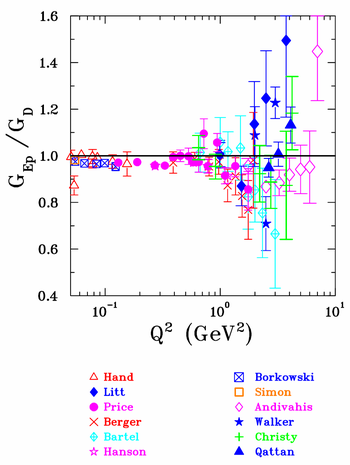
\includegraphics[width=0.9\linewidth]{Pictures/Gep.png}
\caption{Proton electric form factor data from electron scattering. Plot taken from \cite{Perdrisat}.}
\label{fig:Gep}
\end{minipage}%
\begin{minipage}{0.5\textwidth}
\centering
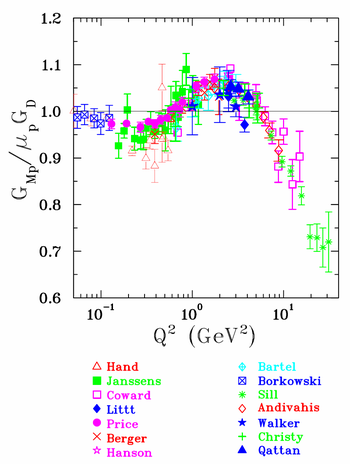
\includegraphics[width=0.9\linewidth]{Pictures/Gmp.png}
\caption{Proton magnetic form factor data from electron scattering. Plot taken from \cite{Perdrisat}.}
\label{fig:Gmp}
\end{minipage}

\end{figure}

In the limit of no target recoil, the cross section for electron-proton scattering is proportional to the square of the sum of the electric and weak scattering amplitudes $\sigma^{r,l}\propto\left|\mathcal{M}\right|^2=\left|\mathcal{M}_{\gamma}+\mathcal{M}_{Z}^{(r,l)}\right|^2$, where r(ight) and l(eft) signify that there is a helicity dependence in the weak neutral amplitudes. The elastic scattering amplitude of electrons from an unpolarized proton target is proportional to the electric and weak currents \cite{Perdrisat}\cite{Goldhaber}
\begin{equation}
\mathcal{M_{\gamma}}=\left(-\frac{1}{q^2}\right)(J_{\gamma}^p)_{\mu}(J_{\gamma}^e)^{\mu},
\label{eq:gamma_scattering_amplitude}
\end{equation}
\begin{equation}
\mathcal{M}_{Z^0}=\left(-\frac{1}{q^2-M_{Z^0}^2}\right)(J_{Z^0}^p)_{\mu}(J_{Z^0}^e)^{\mu}\approx\left(\frac{1}{M_{Z^0}^2}\right)(J_{Z^0}^p)_{\mu}(J_{Z^0}^e)^{\mu},
\label{eq:z_scattering_amplitude}
\end{equation}
where $J^{p(e)}$ are the proton (electron) currents and $q^2$ is the square of the four-momentum transferred from the electron to the proton and $M_{Z^0}$ is the mass of the $Z_0$ boson. The approximation $-q^2+M_{Z^0}^2\rightarrow M_{Z^0}^2$ is valid for low energy scattering. For the electron vertex, the electric and weak neutral currents are given by
\begin{equation}
(J_{\gamma}^{e})_{\mu}=-e\bar u_e(p)\gamma_{\mu}u_e(p^{\prime})
\label{eq:electron_gamma_current}
\end{equation}
\begin{equation}
(J_{Z^0}^{e})_{\mu}=g_z\bar u_e^L(p)\gamma_{\mu}u_e^L(p^{\prime})=\frac{g_z}{2}\bar u_e(p)\gamma_{\mu}(g_V-g_A\gamma^5)u_e(p^{\prime}),
\label{eq:electron_Z_current}
\end{equation}
where $u_e$ are electron spinors, $g_z=g_e/(\sin\theta_W\cos\theta_W)$ is the neutral weak coupling constant, $p~(p^{\prime})$ is the incoming (outgoing) electron four-momentum and $g_V$ and $g_A$ are the vector and axial vector weak charges respectively (see Table \ref{tab:fermion_charges} for weak vector and axial charges of fermions).
The electric and weak neutral proton currents expressed using form factors to account for the proton structure are given by
\begin{equation}
J_{\gamma}^{\mu}=e\bar u(p^{\prime})\left(\gamma^{\mu} F_1^{\gamma}(Q^2) + \frac{i\gamma^{\mu}}{2m_p}\sigma^{\mu\nu}q_{\nu} F_2^{\gamma}(Q^2)\right)u(p),
\label{eq:proton_gamma_current}
\end{equation} 
\begin{equation}
J_{Z}^{\mu}=g_z\bar u(p^{\prime})\gamma^{\mu}\left( F_1^Z(Q^2) + \frac{i\kappa}{2m_p}\sigma^{\mu\nu}q_{\nu} F_2^Z(Q^2) + \gamma^{\mu}\gamma^5 G_A^Z + \gamma^5 G_p^Z\right)u(p),
\label{eq:proton_Z_current}
\end{equation} 
where $F_1^{\gamma}$ and $F_2{\gamma}$ are the the electromagnetic Dirac and Pauli form factors, $F_1^{Z}$ and $F_2^{Z}$ are the weak analogs of the electromagnetic form factors, and $\kappa$ is the anomalous magnetic moment of the proton. The Sachs form factors, most often used for their interpretability, are linear combinations of the Dirac and Pauli form factors and are chosen such that all cross terms cancel in the cross section calculation. In particular $G_E=F_1-\tau\kappa F_2$ and $G_M=F_1+\kappa F_2$. Notice that the weak neutral current requires two further form factors to account for axial terms (terms with a $\gamma^5$) in the cross section: $G_A^{Z}$, the axial-vector proton form factor and $G_P^{Z}$, the pseudoscalar form factor both of which are associated with the axial-vector component of the $Z^0$ interaction \cite{Arrington2007}. These terms violate parity and on this basis are excluded from the electromagnetic current. Neither of these contribute greatly to the ep elastic cross section at the kinematics of the \Qs experiment and can be constrained by other electron scattering data. 

\section{Accessing the Weak Sector via Parity Violation}
Theoretically, the cleanest access to weak sector physics is through neutrinos which, for purposes of experimental physics, only interact weakly\footnote{Since neutrinos have mass they also interact with the Higgs field and are affected by gravity, but these effects are many orders of magnitude weaker than even the weak force.};  however, this also makes neutrino experiments notoriously difficult. In the SM, parity violation is unique to the weak force, making it another gateway to the weak sector. As previously mentioned, the parity operator reverses the sign of all spatial components of a system, that is $P|x,y,z\rangle=|-x,-y,-z\rangle$. The parity operation can be decomposed into a mirror inversion plus a 180 degree rotation around the axis of inversion. Although a mirror only inverts one direction (normal to the mirror surface), yet because the laws of physics are invariant under rotations,\footnote{This implies conservation of angular momentum as shown by Emmy Noether in her famous theorem where she proved that any symmetry in physics implies a conserved quantity.} the parity inversion of a physical process can be accomplished by a mirror inversion. This implies that any difference in measured results between an experiment and its exact mirror experiment must be due to the weak interaction. 


\begin{figure}[ht]
\centering
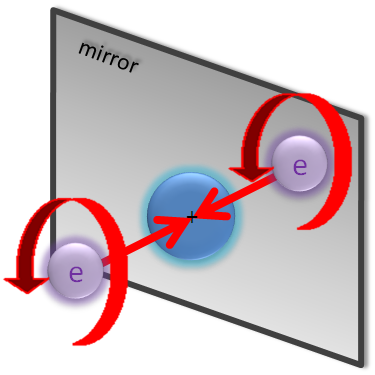
\includegraphics[width=2.5in]{Pictures/parity_inversion.PNG}
\caption{Illustration of parity inversion for \Qs experiment which was accomplished by flipping electron helicity.}
\label{fig:mirror_parity_inversion}
\end{figure}

The \Qs experiment utilized parity violation to determine the weak charge of the proton. This was accomplished by scattering longitudinally polarized electrons off an unpolarized liquid hydrogen target and measuring the difference in elastic scattering rates between electrons of positive and negative helicity. Figure \ref{fig:mirror_parity_inversion} demonstrates that flipping the helicity of longitudinally polarized electrons is equivalent to creating a mirror image experiment. The two processes that contribute to elastic scattering at tree level are shown in Figure \ref{fig:feynman_ep}.

\begin{figure}[t]
\centering

\begin{minipage}{0.5\textwidth}
\centering

\begin{fmffile}{epgammascat}
\begin{fmfgraph*}(35,30)
\fmfbottom{pin,pout}\fmftop{ein,eout}
\fmflabel{$e^-$}{ein}
\fmflabel{$e^-$}{eout}
\fmflabel{$p$}{pin}
\fmflabel{$p$}{pout}
\fmf{boson,label=$\gamma$}{v1,v2}
\fmf{fermion}{pin,v1,pout}
\fmfblob{0.16w}{v1}
\fmf{fermion}{ein,v2,eout}
\fmffreeze
\renewcommand{\P}[3]{\fmfi{plain}{vpath(__#1,__#2) shifted (thick*(#3))}}
\P{pin}{v1}{0.3,-0.8}
\P{pin}{v1}{-0.3,0.8}
\P{v1}{pout}{0.3,0.8}
\P{v1}{pout}{-0.3,-0.8}
\end{fmfgraph*}
\end{fmffile}

\end{minipage}%
\begin{minipage}{0.5\textwidth}
\centering
\begin{fmffile}{epZscat}
\begin{fmfgraph*}(35,30)
\fmfbottom{pin,pout}\fmftop{ein,eout}
\fmflabel{$e^-$}{ein}
\fmflabel{$e^-$}{eout}
\fmflabel{$p$}{pin}
\fmflabel{$p$}{pout}
\fmf{boson,label=$Z$}{v1,v2}
\fmf{fermion}{pin,v1,pout}
\fmfblob{0.16w}{v1}
\fmf{fermion}{ein,v2,eout}
\fmffreeze
\renewcommand{\P}[3]{\fmfi{plain}{vpath(__#1,__#2) shifted (thick*(#3))}}
\P{pin}{v1}{0.3,-0.8}
\P{pin}{v1}{-0.3,0.8}
\P{v1}{pout}{0.3,0.8}
\P{v1}{pout}{-0.3,-0.8}
\end{fmfgraph*}
\end{fmffile}
\end{minipage}
\caption{Tree level Feynman diagrams of neutral electric ($\gamma$-mediated) and neutral weak (Z-mediated) electron-proton scattering.}
\label{fig:feynman_ep}
\end{figure}

The Feynman diagram of elastic ep scattering in Figure \ref{fig:feynman_ep} showing a clean leptonic vertex and a blob at the proton vertex is intended to demonstrate the uncertainty of hadronic interactions that come into play when scattering from a composite object like the proton. In the quark model, the proton is made up of three valence quarks, two up quarks and one down quark, bound together by the strong interaction. As shown in the previous section, the clean interaction equations for fundamental particles (equations \ref{eq:neutral_weak_vertex} and \ref{eq:neutral_em_vertex}) must be modified to account for the internal structure of the proton.

\Qs measured the parity-violating elastic e-p scattering asymmetry by rapidly flipping the helicity of the electron beam. The asymmetry in terms of cross sections of positive and negative helicity electrons on an unpolarized proton target is given by
\begin{equation}
A_{PV}=\frac{\sigma_+-\sigma_-}{\sigma_++\sigma_-},
\label{eq:qw_asymmetry_cx}
\end{equation}
where the cross sections $\sigma$ are averaged over the detector acceptance. At tree level this asymmetry takes the form
\begin{equation}
A_{PV}=\frac{-G_FQ^2}{4\pi \alpha\sqrt{2}}\left[\frac{{\epsilon}G^{\gamma,p}_EG^{Z,p}_E+{\tau}G^{\gamma,p}_MG^{Z,p}_M-\left(1-4sin^2{\theta}_W\right){\epsilon}^{\prime}G^{\gamma,p}_MG^{Z,p}_A}{{\epsilon}(G^{\gamma,p}_E)^2+{\tau}(G^{\gamma,p}_M)^2} \right],
\label{eq:qw_asymmetry}
\end{equation} 
where $G_F$ is the Fermi coupling constant, $\alpha$ is the electromagnetic coupling constant, $Q$ is the four-momentum transfer, $G_E^{\gamma,p}$ and $G_M^{\gamma,p}$ are the Sachs electric and magnetic form factors of the proton and $G_E^{Z,p}$ and $G_M^{Z,p}$ and the analogous form factors for the neutral weak current. $G_A^Z$ is the isovector axial form factor. The kinematic factors $\tau$, $\epsilon$ and $\epsilon^{\prime}$ are defined as follows:
\begin{equation}
\tau=\frac{Q^2}{4m_p^2},~~\epsilon=\frac{1}{1+\left(2+2\tau\tan^2\frac{\theta}{2}\right)},~~\epsilon^{\prime}=\sqrt{\tau(1+\tau)(1-\epsilon^2)},
\label{eq:kinematic_factors}
\end{equation} 
where $m_p$ is the proton rest mass and $\theta$ is the electron scattering angle in the lab frame. All kinematic quantities are acceptance-averaged and the form factors are evaluated at the acceptance-averaged $Q^2$ of \Q.

This asymmetry can be recast as a reduced asymmetry where the leading $Q^2$ dependence has been divided out giving an equation with the proton weak charge $Q_W^p$ as a constant plus terms with higher order dependence on $Q^2$\cite{Erler2005}:
\begin{equation}
\begin{array}{c}
\bar A=\frac{A_{PV}}{A_0}=Q_W^p+Q^2B(Q^2,\theta),\\A_0=\frac{-G_FQ^2}{4\pi\alpha\sqrt{2}}.
\end{array}
\label{eq:reduced_asym}
\end{equation}
$B(Q^2,\theta)$ contains terms with the proton electromagnetic, axial vector and strange quark form factors. In this form the proton weak charge is found by evaluating the reduced asymmetry $\bar A$ at $Q^2=0$.

\section{Radiative Corrections for the \Qs Experiment}
Two types of radiative corrections must be applied to the \Qs data. First, electromagnetic corrections must be applied  for the accurate calculation of experimental kinematics. The extraction of the proton weak charge $Q_W^p$ from the measured asymmetry is accomplished using Equation \ref{eq:reduced_asym}. Although $Q_W^p$ is the value of the reduced asymmetry at $Q^2=0$, all the experimental data were taken at $Q^2>0$. Since all the data are in the second term of the RHS of Equation \ref{eq:reduced_asym} and $Q_W^p$ is given by fitting the data and extrapolating to $Q^2=0$, radiative corrections are vital to proper evaluation of $Q^2$ over the detector acceptance. A small correction must also be applied for depolarization of the electron beam in the target. Second, due to the running of the electric and weak coupling constants, electroweak corrections must be calculated to compare the measurements of Qweak with those of experiments at different kinematics or with different interactions. 

\subsection{Electromagnetic Corrections}
The electron as a light fundamental particle provides a clean probe for particle physics; however, electrons tend to radiate in the presence of target nuclei complicating the interpretation of scattering measurements. The process of correcting electron scattering data (in which only the scattered electron is detected) to account for ``radiative effects'' of the electron beam is a well-established procedure documented by Mo and Tsai\cite{MoAndTsai} in a paper written in 1969 and updated by Tsai\cite{Tsai1971} in 1971.\footnote{Appendix A of Collen Ellis's PhD Thesis {it Measurement of the Strange Quark Contribution to Nucleon Structure through Parity-Violating Electron Scattering}\cite{ColleenEllis} outlines the procedure for electromagnetic radiative corrections for low energy parity-violating electron scattering experiments.} The \Qs experiment measured an asymmetry of scattering rates (cross section difference) between left and right longitudinally polarized electrons on unpolarized protons. Although the detector acceptance allowed a range of kinematic variables, the asymmetry is reported at a set scattering angle and $Q^2$. The data must be corrected for radiative processes in order to accurately report the acceptance-averaged $Q^2$ and scattering angle. For the \Qs experiment there are three basic first-order electromagnetic processes whose contributions must be calculated to accurately report the average energy of the electron at the scattering vertex. These corrections are given the names ``vertex'', ``self-energy'', and ``bremsstrahlung''. A fourth next-to-leading order correction is the vacuum polarization correction which gives the running of the electromagnetic coupling constant\footnote{Although the theory of renormalization is beyond the scope of this thesis, loop diagrams such as the vacuum polarization introduce infinities in calculating scattering amplitudes. These are removed by redefining the coupling constants to depend on the energy scale. Thus, the coupling constants are said to ``run'' with $Q^2$.}. Although a detailed look at radiative corrections is beyond the scope of this thesis, a basic explanation for the four processes can be found in Table \ref{tab:em_radiative_corr}.
\begin{table}[ht]
\caption{Four first order electromagnetic radiative processes contributing to correction for electron-proton scattering.}
\begin{center}
\begin{tabular}{c|p{5cm}|c}\hline
\begin{minipage}{2.0cm}\centering Vertex\\correction\end{minipage}&\begin{minipage}{4.7cm}\vspace{0.25in}Photon emitted before the electron scatters and reabsorbed after scattering\vspace{0.25in}\end{minipage}&
\begin{minipage}{0.25\textwidth}
\centering
\begin{fmffile}{vertex_correction}
\setlength{\unitlength}{0.75cm}
\begin{fmfgraph*}(3,3)
%\begin{fmfgraph*}(20,15)
\fmfright{b}\fmfleft{ein,eout}
\fmf{fermion}{ein,v2,v3,v4,eout}
\fmf{photon}{v3,b} % W line
\fmf{photon,left=0.5,tension=0.2}{v2,v4} % W line
\end{fmfgraph*}
\end{fmffile}
\end{minipage}
\\\hline
\begin{minipage}{2.0cm}\centering Vacuum\\ polarization\end{minipage}&\begin{minipage}{4.7cm}\vspace{0.15in}Virtual photon propagator emits an electron-positron pair which recombine into a virtual photon\end{minipage}\vspace{0.15in} &
\begin{minipage}{0.25\textwidth}
\centering
\begin{fmffile}{vacuum_polarization}
\setlength{\unitlength}{0.75cm}
\begin{fmfgraph*}(3.5,3.2)
\fmfright{b}\fmfleft{ein,eout}
\fmf{phantom,tension=5}{v1,v2}
\fmf{phantom,tension=5}{v3,b}
\fmf{fermion,tension=1.5}{ein,v1,eout}
\fmf{photon}{v1,v2}
\fmf{fermion,left,tension=1.6}{v2,v3,v2}
\fmf{photon}{v3,b}
\end{fmfgraph*}
\end{fmffile}
\end{minipage}
\\\hline

Self energy&\begin{minipage}{4.7cm}\vspace{0.2in}Incoming electron emits and re-absorbs a photon before scattering or scattered electron emits and re-absorbs a photon \end{minipage}\vspace{0.25in}&\begin{minipage}{0.17\textwidth}
\centering
\begin{fmffile}{self_energy1}
\setlength{\unitlength}{0.75cm}
\begin{fmfgraph*}(2.2,3)
%\begin{fmfgraph*}(20,15)
\fmfbottom{in,out}\fmftop{t}
\fmf{plain}{in,v1}
\fmf{fermion}{v1,v2}
\fmf{photon,left,tension=0.0}{v1,v2} 
\fmf{plain}{v2,v3}
\fmf{fermion, tension=0.33}{v3,out}
\fmf{photon}{v3,t} 
\end{fmfgraph*}
\end{fmffile}
\end{minipage}
\vspace{-0.1in}
\begin{minipage}{0.17\textwidth}
\centering
\begin{fmffile}{self_energy2}
\setlength{\unitlength}{0.75cm}
\begin{fmfgraph*}(2.2,3)
%\begin{fmfgraph*}(20,15)
\fmfbottom{in,out}\fmftop{t}
\fmf{fermion,tension=0.33}{in,v1}
\fmf{plain}{v1,v2}
\fmf{fermion}{v2,v3}
\fmf{photon,left,tension=0.0}{v2,v3} 
\fmf{plain}{v3,out}
\fmf{photon}{v1,t} 
\end{fmfgraph*}
\end{fmffile}
\end{minipage}
\vspace{-0.1in}
\\\hline
Bremsstrahlung& \begin{minipage}{4.7cm}Incoming electron or outgoing electron emits a real photon losing energy\end{minipage}\vspace{0.2in}&\begin{minipage}{0.17\textwidth}
\vspace{0.1in}
\centering
\begin{fmffile}{brem1}
\setlength{\unitlength}{0.75cm}
\begin{fmfgraph*}(2.2,3)

\fmfbottom{in,out}\fmftop{t}
\fmfleftn{l}{5}
\fmf{plain}{in,v1}
\fmf{fermion}{v1,v2}
\fmf{plain}{v2,v3}
\fmf{fermion, tension=0.33}{v3,out}
\fmf{photon}{v3,t} 
\fmf{photon, tension=0}{v2,l4} 
\end{fmfgraph*}
\end{fmffile}
\end{minipage}
\begin{minipage}{0.17\textwidth}
\vspace{0.1in}
\centering
\begin{fmffile}{brem2}
\setlength{\unitlength}{0.75cm}
\begin{fmfgraph*}(2.2,3)

\fmfbottom{in,out}\fmftop{t}
\fmfrightn{r}{5}
\fmf{fermion, tension=0.33}{in,v1}
\fmf{plain}{v1,v2}
\fmf{fermion}{v2,v3}
\fmf{photon}{v1,t} 
\fmf{plain}{v3,out}
\fmf{photon, tension=0}{v2,r4} 
\end{fmfgraph*}
\end{fmffile}
\end{minipage}
\\\hline
\end{tabular} 
\end{center}
\label{tab:em_radiative_corr}
\end{table}

\subsection{\label{Sctn:EWcorr}Electroweak Corrections}

Although physical measurements of cross sections involve processes of all orders, results are typically reported at tree level for ease of interpretability. Tree level reporting requires that higher order processes be subtracted off the final result. Thus before the measured Qweak parity-violating asymmetry in Equation \ref{eq:qw_asymmetry_cx} can be interpreted as a tree level process as in Equation \ref{eq:qw_asymmetry}, contributions from higher orders must be calculated and removed.

The weak charge of the proton including one loop radiative corrections can be written as\cite{Erler2003}\cite{Carlson2013}
\begin{equation}
Q_W^p=(1+\Delta\rho+\Delta_e)(1-4\sin^2\hat{\theta}_W+\Delta_e^{\prime})+\Box_{WW}+\Box_{ZZ}+Re\Box_{\gamma Z},
\label{eq:electroweak_rad_corr}
\end{equation}
where $\Delta\rho$ renormalizes the ratio of neutral to charged current interaction strength from the $Z^0$ mass to low energy, $\Delta_e=-\alpha/2\pi$ is an electron vertex correction correction to the axial vector $Zee$ coupling and $\Delta_e^{\prime}$ is a correction to the $\gamma ee$ coupling corresponding to the anapole moment of the electron. The three box corrections are generated by diagrams shown in Figure \ref{fig:box_diagrams}. The box corrections involving only weak interactions, $\Box_{WW}$ and $\Box_{ZZ}$, can be perturbatively calculated due to the large $W$ and $Z^0$ masses\cite{Erler2003}. These two corrections create a cumulative correction of nearly 30\% to $Q_W^p$ but have small associated errors. However, the $\Box_{\gamma Z}$ contribution has a larger uncertainty due to the low $Q^2$ contributions allowed by the photon propagator. The correction $\mathcal{R}e\Box_{\gamma Z}$ has an axial-electron, vector-proton component $\mathcal{R}e\Box_{\gamma Z}^V$ which vanishes as electron energy goes to 0, and a non-vanishing vector-electron, axial-proton component $\mathcal{R}e\Box_{\gamma Z}^A$. Four groups have published calculations of the $\Box_{\gamma Z}^V$ correction at $Q^2=1.165~GeV$, the momentum transfer of the \Qs experiment and obtained similar results (see Table \ref{tab:gamma_Z_correction}). However, the uncertainty on the corrections varies widely with the smallest adding a systematic uncertainty to $Q_W^p$ of $\pm0.00036$. Two published calculations of $\mathcal{R}e\Box_{\gamma Z}^A$ agree within uncertainty on this correction at $E=1.165~GeV$. The correction for $\Box_{\gamma Z}$ and the total correction $\Box_{\gamma Z}^V+\Box_{\gamma Z}^A$ are plotted versus electron energy in Figure \ref{fig:gamma_Z}. 

Table \ref{tab:ew_corrections} shows the size of each correction term in Equation \ref{eq:electroweak_rad_corr} and the error associated with the $\Box_{\gamma Z}$ which dominates the uncertainty of the electroweak radiative corrections.

\begin{figure}[ht]
\centering
\begin{tabular}{ccc}
\begin{fmffile}{wwbox}
\begin{fmfgraph*}(35,25)
  \fmfbottom{i1,d1,o1}%dummy vertex
  \fmftop{i2,d2,o2}
    \fmf{fermion,label=$q$,l.side=right}{i1,v1}
    \fmf{plain,tension=.9}{v1,v2}
    \fmf{fermion,label=$q$,l.side=right}{v2,o1}
    
    \fmf{fermion,label=$e^-$,l.side=left}{i2,v3}
    \fmf{plain,tension=.9}{v3,v4}
    \fmf{fermion,label=$e^-$,l.side=left}{v4,o2}
    \fmf{dashes,label=$W$,tension=0.4,l.side=left}{v1,v3}
    \fmf{dashes,label=$W$,tension=0.4,l.side=right}{v2,v4}
\end{fmfgraph*}

\end{fmffile}&
\begin{fmffile}{zzbox}
\begin{fmfgraph*}(35,25)
  \fmfbottom{i1,d1,o1}%dummy vertex
  \fmftop{i2,d2,o2}
    \fmf{fermion,label=$q$,l.side=right}{i1,v1}
    \fmf{plain,tension=.9}{v1,v2}
    \fmf{fermion,label=$q$,l.side=right}{v2,o1}
    
    \fmf{fermion,label=$e^-$,l.side=left}{i2,v3}
    \fmf{plain,tension=.9}{v3,v4}
    \fmf{fermion,label=$e^-$,l.side=left}{v4,o2}
    \fmf{dashes,label=$Z^0$,tension=0.4,l.side=left}{v1,v3}
    \fmf{dashes,label=$Z^0$,tension=0.4,l.side=right}{v2,v4}
\end{fmfgraph*}

\end{fmffile}&
\begin{fmffile}{gammazbox}
\begin{fmfgraph*}(35,25)
  \fmfbottom{i1,d1,o1}%dummy vertex
  \fmftop{i2,d2,o2}
    \fmf{fermion,label=$q$,l.side=right}{i1,v1}
    \fmf{plain,tension=.9}{v1,v2}
    \fmf{fermion,label=$q$,l.side=right}{v2,o1}
    
    \fmf{fermion,label=$e^-$,l.side=left}{i2,v3}
    \fmf{plain,tension=.9}{v3,v4}
    \fmf{fermion,label=$e^-$,l.side=left}{v4,o2}
    \fmf{photon,label=$\gamma$,tension=0.4,l.side=left}{v1,v3}
    \fmf{dashes,label=$Z^0$,tension=0.4,l.side=right}{v2,v4}
\end{fmfgraph*}
\end{fmffile}
\\
\end{tabular}
\caption{Three box diagrams corresponding to the last three terms in Equation \ref{eq:electroweak_rad_corr}. Crossing diagrams also contribute\cite{Hall2013}.}
\label{fig:box_diagrams} 
\end{figure}
\begin{figure}[ht]
\centering
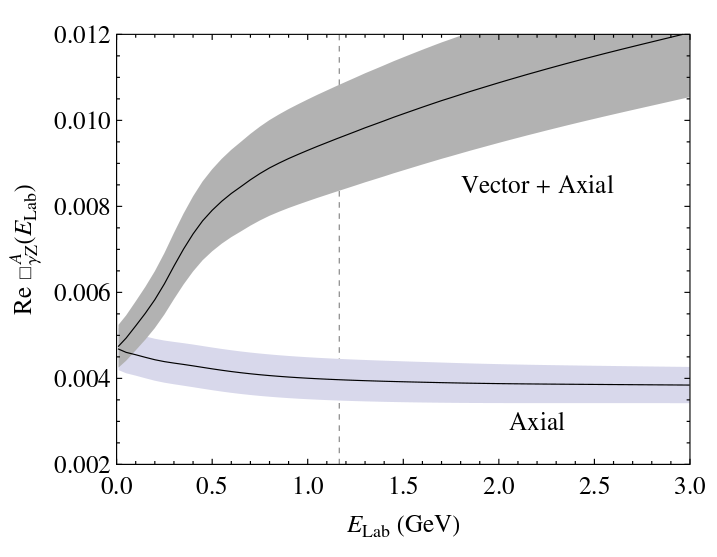
\includegraphics[width=3in]{Pictures/gamma_z.png}
\caption{Correction to $Q_W^p$ from $\Box_{\gamma Z}$ process shown versus electron energy. The axial proton contribution $\mathcal{R}e\Box_{\gamma Z}^A$ is nearly flat at the \Qs kinematics (shown as vertical dashed line), whereas the vector proton contribution $\mathcal{R}e\Box_{\gamma Z}^V$ is energy dependent. Plot taken from Rislow {\it et al.} (2013) \cite{Carlson2013}.}
\label{fig:gamma_Z}
\end{figure}

\begin{table}[ht]
\begin{center}
\caption{Correction to Standard Model $Q_W^p=0.0713(8)$ from axial proton ($\mathcal{R}e\Box_{\gamma Z}^A$) and vector proton ($\mathcal{R}e\Box_{\gamma Z}^V$) components of $\mathcal{R}e\Box_{\gamma Z}$ evaluated at \Qs kinematics $Q^2=1.165~GeV$.}
\label{tab:gamma_Z_correction}
\begin{tabular}{l|c|c}\hline
$\mathcal{R}e\Box_{\gamma Z}^V$&~&~\\
\hline
~&Sibirtsev {\it et al.} (2010) \cite{Sibirtsev2010}&$0.0047_{-0.0004}^{+0.0011}$\\
~&Carlson and Rislow (2011) \cite{Carlson2011}&$0.0057\pm 0.0009$\\
~&Gorchtein {\it et al.} (2011) \cite{Gorchtein2011}&$0.0054\pm 0.0020$\\
~&Hall {\it et al.} (2013) \cite{Hall2013}&$0.00557\pm0.00036$\\
\hline
$\mathcal{R}e\Box_{\gamma Z}^A$&~&~\\
\hline
~&Blunden {\it et al.} (2011) \cite{Blunden2011} &$0.0037_{-0.0004}^{+0.0011}$\\
~&Carlson and Rislow (2013) \cite{Carlson2013}&$0.0040\pm 0.0005$\\
\hline

\end{tabular}
\end{center}
\end{table}

\begin{table}
\begin{center}
\caption{Values for radiative correction terms for $Q_W^p$ found in Equation \ref{eq:electroweak_rad_corr}. Errors are shown for the $\Box_{\gamma Z}$ correction only since its uncertainty dominates the correction. The 2014 Particle Data Group (PDG) values used in the calculations below are as follows: $\alpha = 7.2973525698(24)\times 10^{-3}$, $\hat{\alpha}=\alpha(M_Z)_{\overline{MS}}\approx\frac{1}{128}$,  $\alpha_s(M_Z)=0.1185(6)$ and $\hat s^2=1-\hat c^2=\sin^2\hat{\theta}_W(M_Z)_{(\overline{MS})}=0.23126(5)$.}
\label{tab:ew_corrections}
\begin{tabular}{c|c|c}\hline
Term & Value & Reference\\\hline
$\Delta\rho$ & $0.00833$ & Chetyrkin {\it et al.} (1995) \cite{Chetyrkin1995}\\~&~&~\\
$\Delta_e=\frac{-\alpha}{2\pi}$ & -0.001161 & Erler {\it et al.} (2003) \cite{Erler2003}\\~&~&~\\
$\Delta_e^{\prime}=\frac{-\alpha}{3\pi}(1-4\hat{s}^2)\left(\ln{\frac{M_Z^2}{m_e^2}}+\frac{1}{6}\right)$ & -0.00142 & Erler {\it et al.} (2003) \cite{Erler2003}\\~&~&~\\
$\Box_{WW}=\frac{\hat{\alpha}}{4\pi\hat{s}^2}\left[2+5\left(1-\frac{\alpha_s(M_W^2)}{\pi}\right)\right]$ & $0.01832$ & Erler {\it et al.} (2003) \cite{Erler2003}\\~&~&~\\
$\Box_{ZZ}=\frac{\hat{\alpha}}{4\pi\hat{s}^2\hat{c}^2}\left(\frac{9}{4}-5\hat s^2\right)(1-4\hat s^2 +8\hat s^4)$ & $0.001923$ & Erler {\it et al.} (2003) \cite{Erler2003}\\~&~&~\\
$\Box_{\gamma Z}=\frac{5\hat{\alpha}}{2\pi}(1-4\hat{s}^2)\left(\ln{\frac{M_Z^2}{\Lambda^2}}+C_{\gamma Z}(\Lambda)\right)$ & $0.0093_{-0.0008}^{+0.0015}$ & Hall {\it et al.} (2013) \cite{Hall2013}\\
~& $0.0097\pm0.0014$ & Carlson {\it et al.} (2013) \cite{Carlson2013}\\
\hline
\end{tabular}
\end{center}
\end{table}

Equation \ref{eq:electroweak_rad_corr} shows that $\sin^2\theta_W$ is a function of $Q^2$ which is a key prediction of the SM. As already mentioned, this ``running'' comes from the necessity of including higher order diagrams as $Q^2$ increases. Although $\sin^2\theta_W$ is not an observable and its value depends upon the renormalization scheme chosen, in a given scheme the running of $\sin^2\theta_W$ can be precisely calculated and proves to be a convenient tool for comparing experimental results at different energy scales. In particular, one can compare the SM prediction of the running of $\sin^2\theta_W$ from its precisely determined values near the $Z^0$ resonance. Figure \ref{fig:running_sine_squared_thetaW} shows the predicted running of $\sin^2\theta_W$ from the Z-pole to low energies in the  Modified Minimal Subtraction ($\overline{MS}$) renormalization scheme. A $\pm 4\%$ measurement of $Q_W^p$ at the kinematics of the \Qs experiment would translate to a $\pm 0.3\%$ measurement of $\sin^2\theta_W$ giving a $10\sigma$ test of the SM predicted running from the Z-pole. Deviations from the prediction may be interpreted as signatures of physics beyond the SM, whereas agreement puts significant bounds on certain models of new physics. 
 
\begin{figure}[ht]
\centering
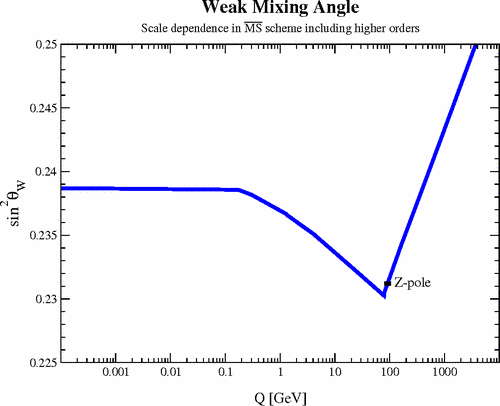
\includegraphics[width=3.0in]{Pictures/running_sine_squared_thetaW.png}
\caption{Standard Model predicted running of $\sin^2\theta_W$ from the Z-pole to low energies evaluated in the $\overline{MS}$ renormalization scheme. The width of the line gives the error in the prediction. Plot taken from Erler {\it et al.} (2013) \cite{Musolf2005}.}
\label{fig:running_sine_squared_thetaW}
\end{figure}

% bibtex thesis
%pdflatex thesis.tex
%mf '\mode=localfont; input brem2'
